\section{Measurement Network Gateway}
\textbf{Introduction}\\
This project details the design and implementation of a robust Measurement Network Gateway deployed on a Xilinx Zynq-7000 SoC (ZedBoard). Designed to bridge the gap between physical instrumentation and remote digital monitoring for Industrial Internet of Things(IIoT) applications , the system acquires high-precision telemetry from a heterogeneous sensor array. This array includes a MAX31865 RTD-to-Digital converter for temperature, Analog-to-Digital Converters (ADC), and digital I/O peripherals. To ensure deterministic hardware sampling without network-induced latency, the software architecture employs a concurrent Producer-Consumer model utilizing POSIX threads (pthreads). A dedicated Sensor Thread manages precise, low-level hardware interactions and pushes timestamped data into a mutex-protected Ring Buffer. Asynchronously, a Server Thread consumes this data, managing TCP/IP network flow control and streaming the telemetry to remote client dashboards. The resulting system provides a scalable, fault-tolerant foundation for real-time remote monitoring, successfully offloading complex data processing to the client while maintaining strict embedded timing constraints.

\begin{figure}[H]
\centering 
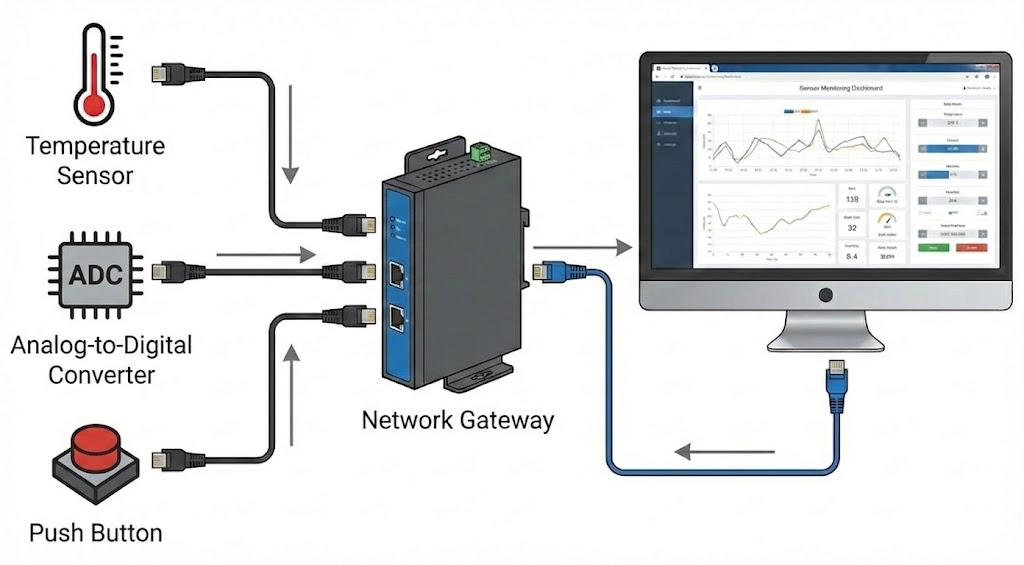
\includegraphics[width = 0.8\textwidth]{media/akshayintro1.png}
\caption{Measurement Network Gateway Interconnection}
\label{fig-akshay1}
\end{figure}

	
\subsection{System Architecture \& Design}
The system is engineered as a distributed network management gateway, designed to facilitate swift and reliable telemetry communication across remote nodes. Operating on a client-server paradigm, the core gateway application is deployed on a Linux operating system running atop the Xilinx Zynq-7000 SoC (ZedBoard), granting it direct interaction with physical hardware components. Conversely, the remote client features a graphical platform utilized to continuously monitor real-time data streams and dynamically configure the distant sensor devices over the TCP/IP network.

\begin{figure}[H]
\centering 
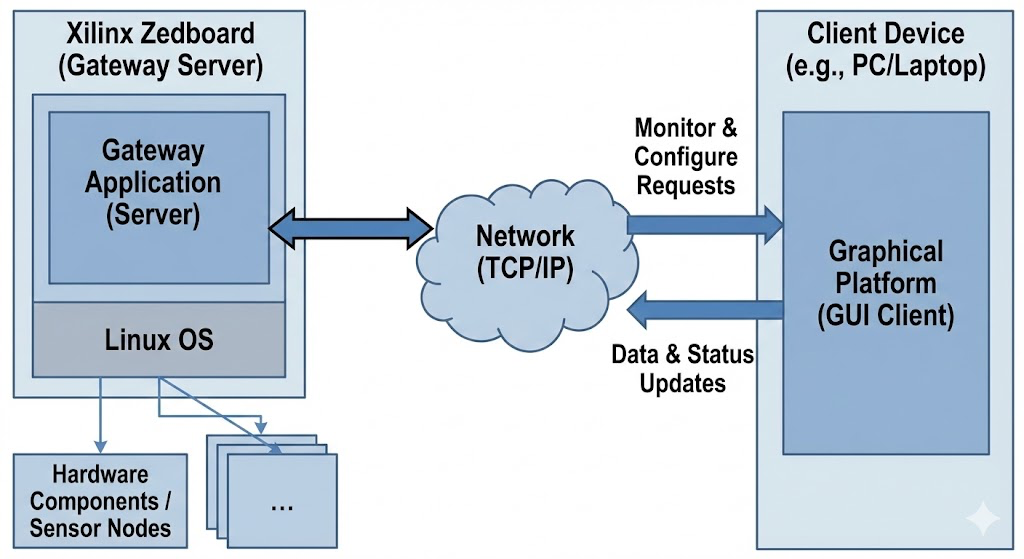
\includegraphics[width = 0.8\textwidth]{media/akshayintro5.png}
\caption{Server-client approach between devices}
\label{fig-akshay2}
\end{figure}
	
	
Concurrent Producer-Consumer Model - To guarantee that data acquisition
remains deterministic and immune to network latency, the internal system
architecture is explicitly built upon a concurrent Producer-Consumer model.
The core of the system is the Sensor Thread, which executes a precise timing
loop to poll hardware peripherals through a custom Linux kernel driver
(\texttt{/dev/meascdd}). By utilizing high-resolution sleep timers and direct
register access, this thread ensures that temperature and analog signals are
sampled at exact user-defined intervals without drift. To achieve this across
multiple independent sensors, the thread employs an "Earliest Deadline First"
scheduling algorithm. It continuously calculates the exact microsecond the
next sensor sample is due and safely yields CPU cycles using \texttt{usleep()}
until that specific deadline is reached.

Decoupling and Shared Memory - To decouple the strict timing requirements of
the hardware from the unpredictable nature of network communication, a
thread-safe Ring Buffer is employed as an intermediate storage mechanism.
Protected by Mutex (Mutual Exclusion) locks, this circular buffer allows the
Sensor Thread to continuously push new data points without blocking, while the
Server Thread (the Consumer) asynchronously retrieves them for transmission.
Crucially, this memory sharing is further optimized using POSIX Condition
Variables (\texttt{pthread\_cond\_t}). Instead of the Server Thread
continuously polling the buffer and wasting CPU resources, it enters a deep
zero-CPU sleep state when the buffer is empty. The exact microsecond the
Sensor Thread commits a new reading to memory, it issues a signal that
instantaneously wakes the Server Thread to batch and transmit the data.

Network Communication and Stability - The Server Thread manages the network
interface, listening on Port 50012 for incoming TCP connections. It handles a
custom command protocol (e.g., \texttt{start}, \texttt{stop},
\texttt{configure}), allowing remote users to dynamically adjust sampling
rates or pause the stream. For instance, the \texttt{configure} command parses
space-delimited string payloads to dynamically update the independent polling
frequencies of the ADC, temperature, and switch components on the fly.

This separation of concerns—isolating the hardware logic from the
communication logic guarantees system stability. Even if the network
connection drops or the client becomes unresponsive, the sensor data
acquisition continues uninterrupted, preventing data loss or system hangs.
Ultimately, this project demonstrates a scalable, industrial-grade solution
for embedded data aggregation, showcasing the effective use of POSIX threads,
event-driven synchronization primitives, and low-level driver interaction on
an embedded Linux platform.

The project is divided into hardware and software parts that fully integrate
later to make project working. In Hardware components, Zynq-7000 ZedBoard,
MAX31865 RTD-to-Digital converter, PmodAD1, RTD-Based Temperature measurement.
On the other hand, Linux kernel is built to integrate hardware information into
the software providing a platform to run the application. It uses ARM core
processors of Xilinx's Zedboard to operate Linux OS. Further, a Remote screen
or Graphical user interface is developed which communicates with the hardware
using Transmission Control Protocol (TCP/IP).


%


\subsection{Architectural Overview \& Userspace Bridging}
The module serves as the critical translation layer between the
high-level multithreaded server logic and the physical hardware of the
Xilinx ZedBoard. Because Linux strictly separates userspace applications
from physical hardware memory, this module acts as a secure bridge
utilizing standard POSIX file operations. By hiding complex
bit-shifting, SPI polling loops, and timeout safeguards behind simple
functions like \texttt{TempRead()} and \texttt{GetADC()}, it allows the
higher-level multithreaded architecture to remain clean, fast, and
entirely focused on timing and network transmission. The
\texttt{sensor\_read.c} file is a robust, fault-tolerant module.

\begin{minted}[bgcolor = lightgray, tabsize = 4, breaklines]{c}
    #include <fcntl.h>
    #include <unistd.h>
    #include "measdev.h"
    #include "sensor_read.h"
    MeasObj_struct TF_Obj_Snd, TF_Obj_Rcv;
\end{minted}


\begin{itemize}
    \item \textbf{Communication Struct (\texttt{MeasObj\_struct})}: The
          application cannot read physical memory addresses directly.
          Instead, it packs commands into \texttt{TF\_Obj\_Snd} (Transmit)
          and pushes them into the file descriptor \texttt{fd} pointing to
          the custom kernel driver (\texttt{/dev/meascdd}). The hardware
          response is then retrieved via \texttt{TF\_Obj\_Rcv}.

    \item \textbf{Modularity}: By hiding complex bit-shifting and SPI
          polling loops inside this module, the main sensor thread remains
          clean, lightweight, and hardware-agnostic.
\end{itemize}

\subsubsection{Low-Level SPI Protocol Management}
Interacting with the MAX31865 temperature chip requires precise,
timing-aware SPI bus transactions. The functions \texttt{MaxRead()} and
\texttt{MaxWrite()} are engineered to handle the physical delays of
hardware communication safely using strict polling loops and timeout
safeguards.

\subsubsection*{The MaxRead Function}
\begin{minted}[bgcolor = lightgray, tabsize = 4, breaklines]{c}
unsigned int MaxRead(int fd, unsigned int mreg)
{
    unsigned int xdata;
    int k;

    mreg <<= 8;
    TF_Obj_Snd.rnum = 1;
    TF_Obj_Snd.rvalue = mreg;
    write(fd, &TF_Obj_Snd, MEASOBJ_SIZE);
\end{minted}

\subsubsection*{Command Preparation \& Transfer: }
The target register address is shifted left by 8 bits (\texttt{mreg <<= 8}) and pushed to the driver (\texttt{rnum = 1}).
\begin{minted}[bgcolor = lightgray, tabsize = 4, breaklines]{c}
    k = 0;
    xdata = 0xc0000000;
    do {
        TF_Obj_Snd.rnum = REGNUM_ID;
        TF_Obj_Snd.rvalue = 1;
        write(fd, &TF_Obj_Snd, MEASOBJ_SIZE);
        k++;
        read(fd, &TF_Obj_Rcv, MEASOBJ_SIZE); // Read response from LKM
        xdata = TF_Obj_Rcv.rvalue;
    } while (((xdata & 0x01) == 0) && (k < 1000));
\end{minted}

\subsubsection*{The Polling State Machine \& Timeout: }
The code enters a strict \texttt{do-while} loop, querying the driver
for a status update. It checks whether the hardware is ready by
inspecting the lowest bit (\texttt{xdata \& 0x01}). The loop is capped
at \texttt{k < 1000} iterations to prevent system freezes if the
physical wire is disconnected.

\begin{minted}[bgcolor = lightgray, tabsize = 4, breaklines]{c}
    if (k >= 1000) {
        printf(" *** MaxRead timeout.");
    } else {
        TF_Obj_Snd.rnum = REGNUM_ID;
        TF_Obj_Snd.rvalue = 2;
        write(fd, &TF_Obj_Snd, MEASOBJ_SIZE);
        read(fd, &TF_Obj_Rcv, MEASOBJ_SIZE); // Read response from LKM
        xdata = TF_Obj_Rcv.rvalue;
        xdata &= 0x0ff;
    }
    return xdata;
}
\end{minted}

\subsubsection*{Data Extraction: }
Once ready, it reads the final value and masks it (xdata \&= 0x0ff) to ensure a clean 8-bit payload.

\subsubsection{The MaxWrite Function}
To signal a write operation over SPI, the highest bit of the register
address is set to \texttt{1} (\texttt{mreg |= 0x080}).

\begin{minted}[bgcolor = lightgray, tabsize = 4, breaklines]{c}
void MaxWrite(int fd, unsigned int mreg, unsigned int msend)
{
    unsigned int transm_data, xdata;
    int k;

    mreg |= 0x080;
    transm_data = (mreg << 8) | (msend & 0x0ff);
    TF_Obj_Snd.rnum = 1;
    TF_Obj_Snd.rvalue = transm_data;
    write(fd, &TF_Obj_Snd, MEASOBJ_SIZE);
\end{minted}

\subsubsection*{Payload Construction: }
The 16-bit payload combines the register address and the data byte:
\texttt{(mreg << 8) | (msend \& 0x0ff)}. Identical to \texttt{MaxRead()},
it uses the 1000-iteration polling loop to guarantee the write command
was physically clocked into the sensor.

\begin{minted}[bgcolor = lightgray, tabsize = 4, breaklines]{c}
     k = 0;
    xdata = 0xc0000000;
    do {
        TF_Obj_Snd.rnum = REGNUM_ID;
        TF_Obj_Snd.rvalue = 1;
        write(fd, &TF_Obj_Snd, MEASOBJ_SIZE);
        k++;
        read(fd, &TF_Obj_Rcv, MEASOBJ_SIZE); // Read response from LKM
        xdata = TF_Obj_Rcv.rvalue;
    } while (((xdata & 0x01) == 0) && (k < 1000));
    
    if (k >= 1000) {
        printf(" *** MaxWrite timeout.");
    }
}
\end{minted}

\subsubsection*{MAX31865 Temperature Sensor API}
This section wraps the complex \texttt{MaxRead()} and \texttt{MaxWrite()}
logic into three simple lifecycle functions tailored specifically for the
MAX31865 RTD-to-Digital converter.

\paragraph{Initialization (TempPowerUp): }
Writes the hex value \texttt{0xC1} to the configuration register. This turns on VBIAS, enables Auto-Conversion mode, and enables the 50Hz hardware noise rejection filter. A calculated \texttt{usleep(75000)} allows the analog circuitry 75ms to settle.
\begin{minted}[bgcolor = lightgray, tabsize = 4, breaklines]{c}
int TempPowerUp(int fd)
{
    ssize_t ret;

    TF_Obj_Snd.rnum   = 0;
    TF_Obj_Snd.rvalue = 0x022;
    ret = write(fd, &TF_Obj_Snd, MEASOBJ_SIZE);
    if (ret < 0) { perror("Sensor Initialization Failed"); return -1; }

    MaxWrite(fd, 0x00, 0xC1);   // VBIAS=ON, AutoConv=ON, 2-wire, 50Hz
    usleep(75 * 1000);           // 10ms VBIAS settle + 65ms first conversion
    printf("MAX31865 powered up in auto-conversion mode\n");
    return 1;
}
\end{minted}



\paragraph{Data Retrieval (TempRead): }
Fetches the Most Significant Byte (MSB) and Least Significant Byte (LSB). It evaluates \texttt{if (lsb \& 0x01)} to detect hardware faults (like a broken wire) to prevent broadcasting false data. If valid, the 16-bit integer is reassembled and shifted right by 1 (\texttt{>> 1}) to discard the fault bit, isolating the true 15-bit ADC count.
\begin{minted}[bgcolor = lightgray, tabsize = 4, breaklines]{c}
int TempRead(int fd, int *output_raw)
{
    unsigned int msb = MaxRead(fd, 0x01);
    unsigned int lsb = MaxRead(fd, 0x02);

    if (lsb & 0x01) {
        printf("MAX31865 fault: 0x%02X\n", MaxRead(fd, 0x07));
        return -1;
    }

    *output_raw = (int)((((msb & 0xFF) << 8) | (lsb & 0xFF)) >> 1);
    return 1;
}
\end{minted}


\paragraph{Safe Termination (TempShutdown): }
Writes \texttt{0x01} to disable VBIAS and save power during system shutdown.
\begin{minted}[bgcolor = lightgray, tabsize = 4, breaklines]{c}
void TempShutdown(int fd)
{
    MaxWrite(fd, 0x00, 0x01);
    printf("MAX31865 powered down\n");
}
\end{minted}

\subsubsection{Dual-Channel Analog-to-Digital (ADC) Processing}
The GetADC function communicates with the ZedBoard's ADC peripherals, handling two separate voltage channels simultaneously.
\begin{minted}[bgcolor = lightgray, tabsize = 4, breaklines]{c}
void GetADC(int fd, unsigned int *adc0_out, unsigned int *adc1_out)
{
    int  ccount;
    unsigned int xstatus, adc0, adc1;
    TF_Obj_Snd.rnum = 4;        // start conversion
    TF_Obj_Snd.rvalue = 0;
    write(fd, &TF_Obj_Snd, MEASOBJ_SIZE);
    ccount = 0;
    
    do {
        ccount++;
        read(fd, &TF_Obj_Rcv, MEASOBJ_SIZE);        // Read response from LKM
        xstatus = TF_Obj_Rcv.rvalue;
    } while ((xstatus == 0) && (ccount < 10000000));
\end{minted}

\paragraph{Trigger and Wait: }
Writes a \texttt{0} to \texttt{rnum = 4} to signal the FPGA to sample analog voltages. An extended polling loop (\texttt{ccount < 10000000}) provides the hardware ample time to charge its internal capacitors and complete the conversion.
\begin{minted}[bgcolor = lightgray, tabsize = 4, breaklines]{c}
       TF_Obj_Snd.rnum = REGNUM_ID;
    TF_Obj_Snd.rvalue = 5;      // ADC status register
    write(fd, &TF_Obj_Snd, MEASOBJ_SIZE);
    read(fd, &TF_Obj_Rcv, MEASOBJ_SIZE);        // Read response from LKM
    
    adc1 = TF_Obj_Rcv.rvalue;
    adc0 = adc1 & 0x0fff;
    adc1 >>= 16;
    *adc0_out = adc0;
    *adc1_out = adc1;
}
\end{minted}

\paragraph{Bitwise Separation: }
The hardware returns a highly optimized 32-bit package containing both readings.
\begin{itemize}
    \item \textbf{ADC0 Extraction:} Applies a bitwise AND mask (\texttt{adc1 \& 0x0fff}) to isolate the lowest 12 bits (values 0--4095).
    \item \textbf{ADC1 Extraction:} Applies a bitwise right-shift (\texttt{adc1 >>= 16}) to push the upper 12 bits down to the bottom, safely separating the second reading.
\end{itemize}

\subsubsection{Digital I/O (Switches, Buttons, and LEDs)}
This section maps the physical user interface of the ZedBoard directly into the software.

\paragraph{Switch Acquisition (ReadSwitch): }
Queries the main status register. Applying an \texttt{\& 0xff} (Binary: \texttt{1111 1111}) mask to the 32-bit return value instantly zeroes out irrelevant upper bits, isolating the exact ON/OFF states of the 8 physical sliding switches.

\begin{minted}[bgcolor = lightgray, tabsize = 4, breaklines]{c}
    unsigned int ReadSwitch(int fd)
{
    TF_Obj_Snd.rnum = REGNUM_ID;
    TF_Obj_Snd.rvalue = 0;
    write(fd, &TF_Obj_Snd, MEASOBJ_SIZE);
    read(fd, &TF_Obj_Rcv, MEASOBJ_SIZE);
    
    return (TF_Obj_Rcv.rvalue) & 0xff;
}
\end{minted}

\subsubsection*{Push Button Acquisition (ReadButton): }
Queries the exact same register but shifts the result right by 8 bits (\texttt{>> 8}). Because there are only 5 push buttons, it applies a strict \texttt{\& 0x1f} (Binary: \texttt{0001 1111}) mask to isolate just those 5 states.
\begin{minted}[bgcolor=lightgray, tabsize=4, breaklines]{c}
unsigned int ReadButton(int fd)
{
    TF_Obj_Snd.rnum = REGNUM_ID;
    TF_Obj_Snd.rvalue = 0;
    write(fd, &TF_Obj_Snd, MEASOBJ_SIZE);
    read(fd, &TF_Obj_Rcv, MEASOBJ_SIZE);

    return ((TF_Obj_Rcv.rvalue) >> 8) & 0x1f;
}
\end{minted}

\subsubsection*{LED Control (LedWrite): }
Pushes a standard 8-bit hex payload to \texttt{rnum = 0}. The FPGA hardware interprets this payload and instantly illuminates the corresponding sequence of the 8 onboard yellow LEDs, providing real-time visual feedback.

\begin{minted}[bgcolor=lightgray, tabsize=4, breaklines]{c}
void LedWrite(int fd, uint8_t LED_hex_Value)
{
    ssize_t ret;
    TF_Obj_Snd.rnum   = 0;       // write reg0 (lower 8 bits = uzLED)
    TF_Obj_Snd.rvalue = (unsigned int)LED_hex_Value;
    ret = write(fd, &TF_Obj_Snd, MEASOBJ_SIZE);
    if (ret < 0) perror("LED writing failed");
}
\end{minted}








\clearpage 


\section{Network Communication}
\subsection{Transmission Control Protocol (TCP)}
It is one of the most fundamental protocols of the internet. If the internet is a massive highway system, IP (Internet Protocol) is the GPS routing the trucks, and TCP is the logistics company ensuring every single package arrives intact, in the correct order, and confirming delivery with the sender.
The Transmission Control Protocol (TCP) is a foundational communication protocol of the modern internet. While the Internet Protocol (IP) manages the addressing and routing of packets across disparate networks, TCP operates at the transport layer to ensure the reliable, ordered, and error-checked delivery of data streams between applications communicating over an IP network.

\subsection{Core Characteristics of TCP}
TCP was specifically engineered to mitigate the inherent unreliability of physical network infrastructure, where latency, packet loss, and hardware limitations are commonplace. By operating transparently over this variable underlying layer, TCP provides applications with a robust and dependable communication channel.
\begin{itemize}
\item \textbf{Connection-Oriented:} Prior to any data transmission, TCP establishes a formal session between endpoints using a protocol known as the three-way handshake. This synchronizes sequence numbers and operational parameters between the client and server.
\item \textbf{Reliable Delivery:} TCP employs a strict system of acknowledgments and timeouts. If a transmitted segment is not acknowledged by the receiver within a specified timeframe, TCP assumes the packet was lost and automatically retransmits the data, guaranteeing complete delivery.
\item \textbf{In-Order Delivery:} Because individual IP packets may traverse different network paths and arrive out of sequence, TCP affixes a sequence number to each segment. This allows the receiving network stack to reassemble the payload in the precise order it was originally transmitted.
\item \textbf{Error Checking:} Each TCP segment includes a cryptographic checksum in its header. The receiver independently calculates the checksum of the incoming data and compares it to this field to detect bit-level corruption that may have occurred during transit.
\item \textbf{Flow Control:} To prevent a high-bandwidth sender from overwhelming a receiver with limited processing capacity or memory, TCP utilizes a sliding window mechanism. The receiver continuously advertises its available buffer space, dictating the maximum volume of unacknowledged data the sender is permitted to transmit at any given moment.
\item \textbf{Congestion Control:} TCP implements advanced algorithms to detect network-wide congestion (typically inferred from dropped packets or delayed acknowledgments). Upon detecting network saturation, the protocol dynamically throttles its transmission rate to alleviate strain on intermediary routers and prevent systemic network collapse.
\end{itemize}



\clearpage
\subsection{TCP Server-Client Connection}
\begin{figure}[H]
\centering 
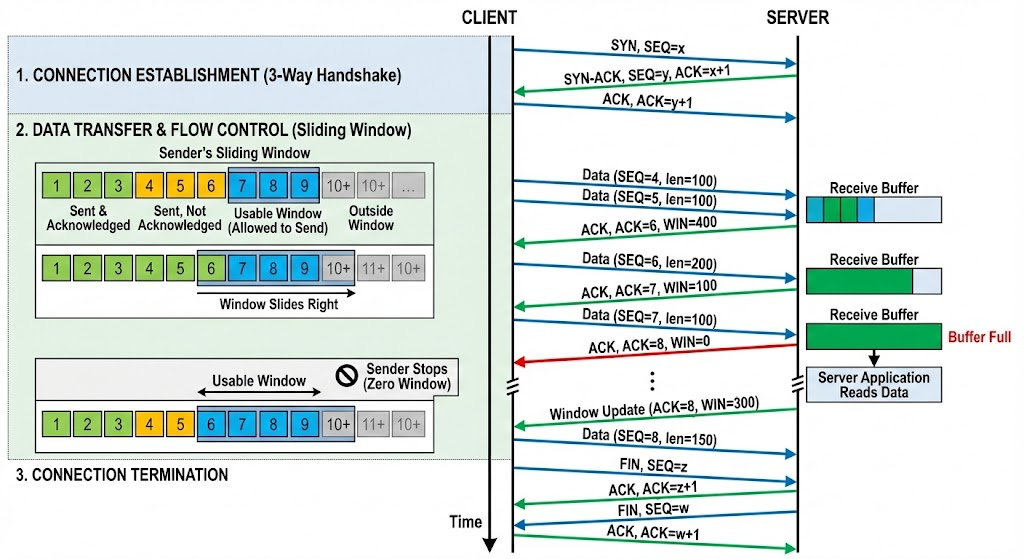
\includegraphics[width = 0.9\textwidth]{media/akshayintro8.png}
\caption{TCP Client-Server setup connection}
\label{fig-akshyintro3}
\end{figure}
	
The Transmission Control Protocol (TCP) provides the foundation for reliable network communication. In the context of your embedded gateway system, this protocol governs the stable, continuous streaming of sensor data from the server to the client dashboard. The TCP connection lifecycle is structured around three primary phases:
	

\textbf{1. Connection Establishment :} Prior to any data transmission, the client and server must synchronize their connection states. The client initiates this process by transmitting a SYN (Synchronize) packet containing an initial sequence number. The server allocates the necessary resources and responds with a SYN-ACK packet, which the client then formally acknowledges (ACK). This establishes a secure, bidirectional communication channel.

\textbf{2. Data Transfer and Flow Control :} To prevent high-speed data streams from overwhelming the receiving system's memory, TCP employs a dynamic "Sliding Window" protocol.

\begin{itemize}
\item Buffer Management: The receiving server allocates a finite memory buffer for incoming data. With every acknowledgment (ACK) it sends back to the client, it also advertises its current available buffer capacity using the Window Size (WIN) parameter.
\item State Tracking: The sender categorizes data into strict states (acknowledged, in-transit, permitted to send, and blocked) and restricts its transmission output to fit within the receiver's advertised window.
\item The "Zero Window" State: If the receiver's buffer reaches maximum capacity, it broadcasts a WIN=0. To prevent data loss, the sender immediately halts transmission. Once the receiving application processes the buffered data, the receiver issues a Window Update with a non-zero value, allowing transmission to resume.
\end{itemize}

\textbf{3. Connection Termination:} Upon completing the data transfer, the session is gracefully dismantled to ensure no in-transit data is corrupted or lost. Both the client and server perform a reciprocal exchange of FIN (Finish) and ACK packets. Once both sides have confirmed termination, the connection is formally closed, and the operating system releases the associated ports and memory resources.